\chapter{Analysis of molecular variance (AMOVA)}

We've already encountered $\pi$, the nucleotide diversity in a
population, namely
\[
\pi = \sum_{ij} x_ix_j \delta_{ij} \quad ,
\]
where $x_i$ is the frequency of the $i$th haplotype and $\delta_{ij}$
is the fraction of nucleotides at which haplotypes $i$ and $j$
differ.\footnote{When I introduced nucleotide diversity before, I
  defined $\delta_{ij}$ as the {\it number\/} of nucleotides that
  differ between haplotypes $i$ and $j$. It's a little easier for what
  follows if we think of it as the {\it fraction\/} of nucleotides at
  which they differ instead. It's really easy to convert between the
  two. If $\delta^*{ij}$ is the {\it number\/} of nucleotides that
  differ between haplotypes $i$ and $j$ and $N$ is the length of the
  haplotype sequence, then $\delta_{ij} = \delta^*{ij}/N$. Of course,
  if we wanted to get fancy we could use a Bayesian approach to
  estimate $\delta_{ij}$, but we'll avoid that complication in what
  follows.} It shouldn't come to any surprise to you that just as
there is interest in partitioning diversity within and among
populations when we're dealing with simple allelic variation, i.e.,
Wright's $F$-statistics, there is interest in partitioning diversity
within and among populations when we're dealing with nucleotide
sequence or other molecular data. The approach I'm going to describe
is known as Analysis of Molecular VAriance
(AMOVA)~\cite{Excoffier-etal92}. We'll see later that AMOVA can be
used very generally to partition variation when there is a distance we
can use to describe how different alleles are from one another, but
for now, let's stick with nucleotide sequence data and think of
$\delta_{ij}$ simply as the fraction of nucleotide sites at which two
sequences differ.\index{nucleotide diversity}

\section*{Analysis of molecular variance
  (AMOVA)}\index{AMOVA}\index{Analysis of molecular variance}

The notation now becomes just a little bit more complicated. We will
now use $x_{ik}$ to refer to the frequency of the $i$th haplotype in
the $k$th population. Then
\[
x_{i\cdot} = \frac{1}{K}\sum_{k=1}^K x_{ik}
\]
is the mean frequency of haplotype $i$ across all populations, where
$K$ is the number of populations. We can now define
\begin{eqnarray*}
\pi_t &=& \sum_{ij} x_{i\cdot}x_{j\cdot} \delta_{ij} \\
\pi_s &=& \frac{1}{K}\sum_{k=1}^K\sum_{ij} x_{ik}x_{jk}\delta_{ij} \quad ,
\end{eqnarray*}
where $\pi_t$ is the nucleotide sequence diversity across the entire
set of populations and $\pi_s$ is the average nucleotide sequence
diversity within populations. Then we can define\index{nucleotide diversity!partitioning}
\begin{equation}
\Phi_{st} = \frac{\pi_t - \pi_s}{\pi_t} \quad ,
\label{eq:phi-st}
\end{equation}
which is the direct analog of Wright's $F_{st}$ for nucleotide
sequence diversity. Why? Well, that requires you to remember stuff we
covered about two months ago.\index{Phi-st@$\Phi_{st}$}\index{AMOVA}

To be a bit more specific, refer back to the 
notes on $F_{ST}$.\footnote{You can find the online version here, if
  you don't have them handy: \url{http://darwin.eeb.uconn.edu/eeb348-notes/genetic-structure.pdf}.}.
When you do, you'll see that we defined
\[
F_{IT} = 1 - \frac{H_i}{H_t} \quad ,
\]
where $H_i$ is the average heterozygosity in individuals and $H_t$ is
the expected panmictic heterozygosity. Defining $H_s$ as the average
panmictic heterozygosity within populations, we then observed that
\begin{eqnarray*}
1 - F_{IT} &=& \frac{H_i}{H_t} \\
           &=& \frac{H_i}{H_s}\frac{H_s}{H_t} \\
           &=& (1 - F_{IS})(1 - F_{ST}) \quad .
\end{eqnarray*}
We can rearrange that equation a bit to solve for $F_{ST}$ in terms of
$F_{IT}$ and $F_{IS}$.

\begin{eqnarray*}
1-F_{ST} &=& \frac{1-F_{IT}}{1-F_{IS}} \\
F_{ST} &=&
\frac{\left(1-F_{IS}\right)-\left(1-F_{IT}\right)}{1-F_{IS}} \\
&=& \frac{\left(H_i/H_s\right) - \left(H_i/H_t\right)}{H_i/H_s} \\
&=& \frac{\left(1/H_S\right) - \left(1/H_t\right)}{1/H_s} \\
&=& 1 - \frac{1/H_t}{1/H_S} \\  
&=& 1 - \frac{H_s}{H_t} \quad .
\end{eqnarray*}
In short, another way to think about $F_{ST}$ is
\begin{equation}
F_{ST} = \frac{H_t - H_s}{H_t} \quad .
\label{eq:f-st}
\end{equation}
Now if you compare equation~(\ref{eq:phi-st}) and
equation~(\ref{eq:f-st}), you'll see the analogy.

So far I've motivated this approach by thinking about $\delta_{ij}$ as
the fraction of sites at which two haplotypes differ and $\pi_s$ and
$\pi_t$ as estimates of nucleotide diversity. But nothing in the
algebra leading to equation~(\ref{eq:phi-st}) requires that
assumption. Excoffier et al.~\cite{Excoffier-etal92} pointed out that
other types of molecular data can easily be fit into this
framework. We simply need an appropriate measure of the ``distance''
between different haplotypes or alleles. Even with nucleotide
sequences the appropriate $\delta_{ij}$ may reflect something about
the mutational pathway likely to connect sequences rather than the raw
number of differences between them. For example, the distance might be
a Jukes-Cantor distance or a more general distance measure that
accounts for more of the properties we know are associated with
nucleotide substitution. The idea is illustrated in
Figure~\ref{fig:amova-procedure}.

Notice that when we're partitioning diversity with AMOVA, we're using
the word ``diversity'' in a different sense than we did with
$F$-statistics. With $F$-statistics we were thinking about diversity
solely in terms of allele frequency differences. With AMOVA we're
thinking about diversity in terms of a combination of haplotype
frequency differences {\it and\/} a measure of how different{\dash}how
distant{\dash} those haplotypes are from one another.

Once we have $\delta_{ij}$ for all pairs of haplotypes or alleles in
our sample, we can use the ideas lying behind
equation~(\ref{eq:phi-st}) to partition diversity{\dash}the average
distance between randomly chosen haplotypes or alleles{\dash}into
within and among population components.\footnote{As with
  $F$-statistics, the actual estimation procedure is more complicated
  than I describe here. Standard approaches to AMOVA use method of
  moments calculations analogous to those introduced by Weir and
  Cockerham for $F$-statistics~\cite{WeirCockerham84}. Bayesian
  approaches are possible, but they are not yet widely
  available~(meaning, in part, that I know how to do it, but I haven't
  written the necessary software yet). Gompert et
  al.~\cite{Gompert-etal-2010} describe one approach for Bayesian
  AMOVA from pooled DNA sequences obtained from high-throughput
  sequencing.} This procedure for partitioning diversity in molecular
markers is referred to as an analysis of molecular variance or AMOVA
(by analogy with the ubiquitous statistical procedure analysis of
variance, ANOVA). Like Wright's $F$-statistics, the analysis can
include several levels in the hierarchy.

\begin{figure}
\begin{center}
\resizebox{!}{8cm}{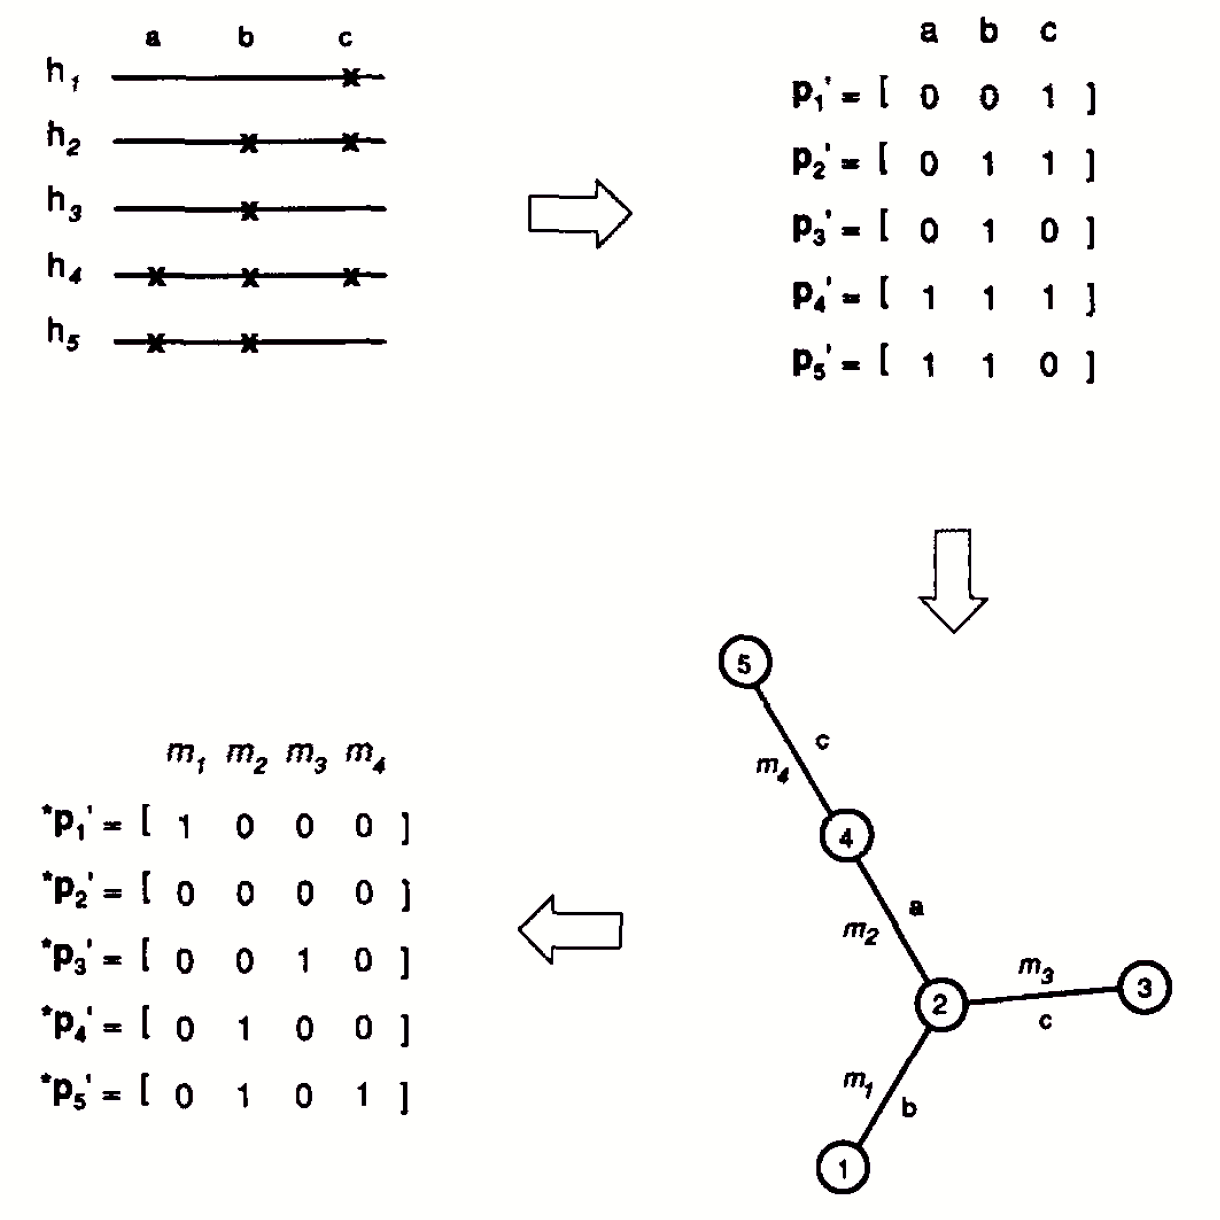
\includegraphics{amova-procedure.eps}}
\end{center}
\caption{Converting raw differences in sequence (or presence and
  absence of restriction sites) into a minimum spanning tree and a
  mutational measure of distance for an analysis of molecular variance~(from~\cite{Excoffier-etal92}).}\label{fig:amova-procedure}
\end{figure}

\section*{An AMOVA example}\index{AMOVA!example}

Excoffier et al.~\cite{Excoffier-etal92} illustrate the approach by
presenting an analysis of restriction haplotypes in human mtDNA. They
analyze a sample of 672 mitochondrial genomes representing two
populations in each of five regional
groups~(Figure~\ref{fig:amova-sample-locations}). They identified 56
haplotypes in that sample. A minimum spanning tree illustrating the
relationships and the relative frequency of each haplotype is
presented in Figure~\ref{fig:amova-haplotypes}.

\begin{figure}
\begin{center}
\resizebox{!}{6cm}{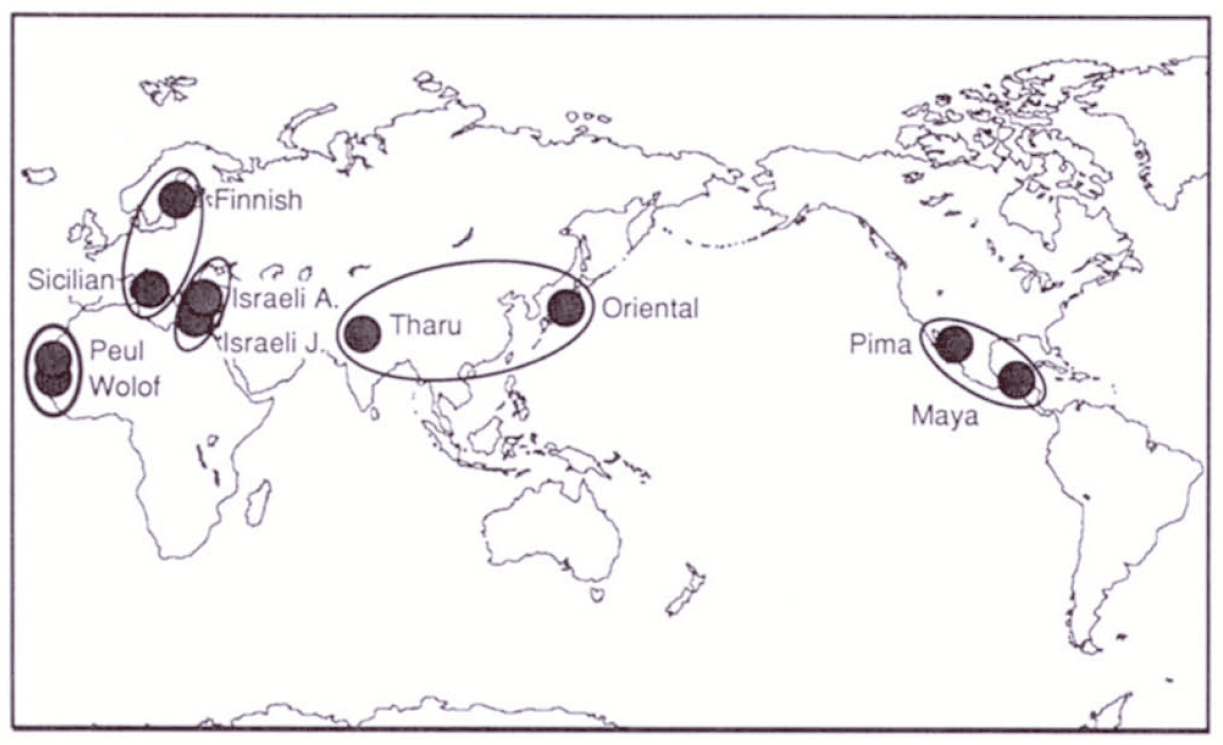
\includegraphics{amova-sample-locations.eps}}
\end{center}
\caption{Locations of human mtDNA samples used in the example
  analysis~(from~\cite{Excoffier-etal92}).}\label{fig:amova-sample-locations}
\end{figure}

\begin{figure}
\begin{center}
\resizebox{!}{6cm}{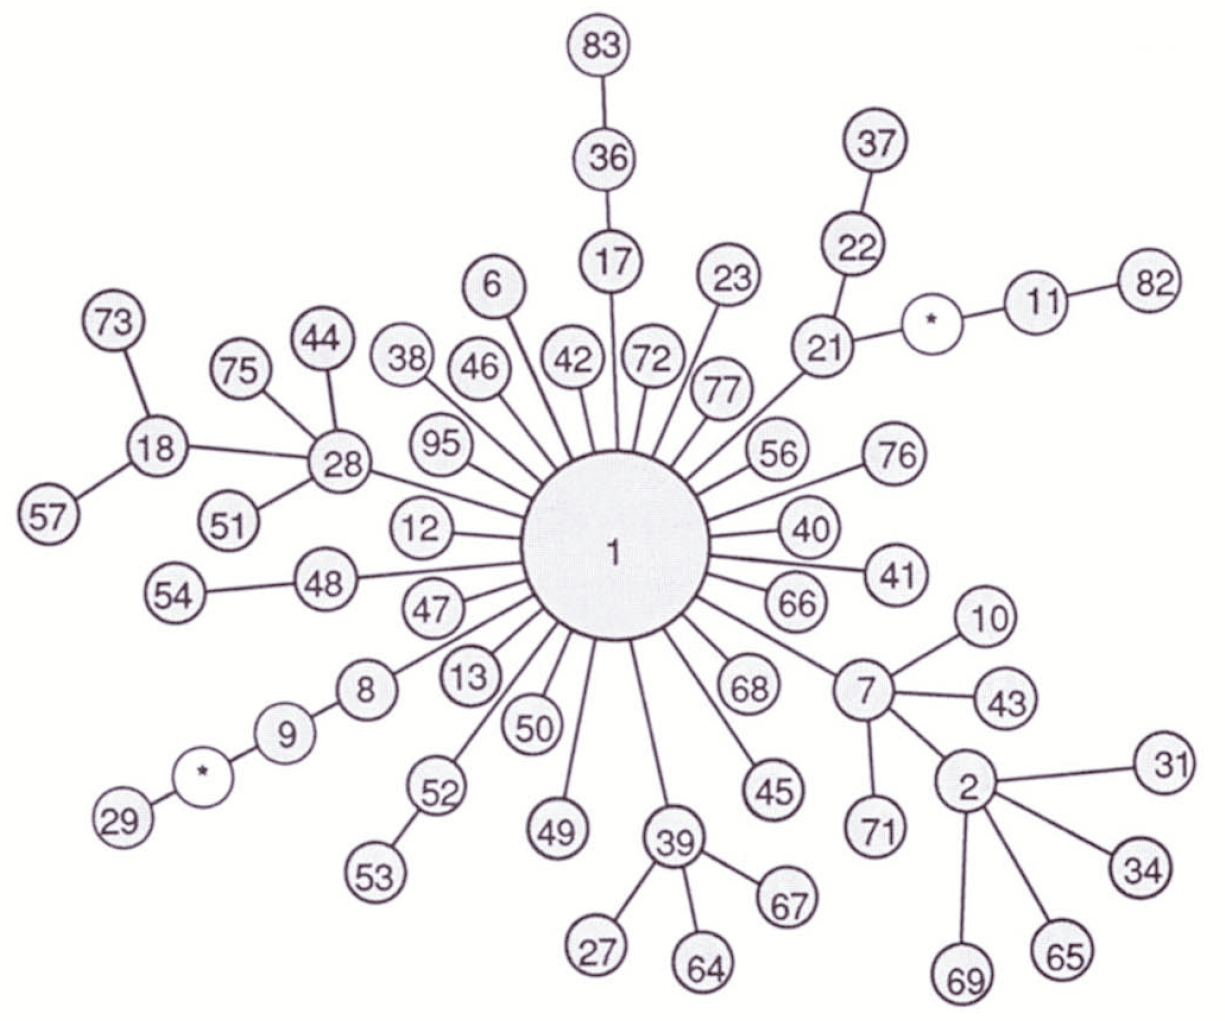
\includegraphics{amova-haplotypes.eps}}
\end{center}
\caption{Minimum spanning network of human mtDNA samples in the
  example. The size of each circle is proportional to its
  frequency~(from~\cite{Excoffier-etal92}).}\label{fig:amova-haplotypes}
\end{figure}

It's apparent from Figure~\ref{fig:amova-haplotypes} that haplotype 1
is very common. In fact, it is present in substantial frequency in
every sampled population. An AMOVA using the minimum spanning network
in Figure~\ref{fig:amova-haplotypes} to measure distance produces the
results shown in Table~\ref{table:amova-results}. Notice that there is
relatively little differentiation among populations within the same
geographical region ($\Phi_{SC} = 0.044$). There is, however,
substantial differentiation among regions ($\Phi_{CT} = 0.220$). In
fact, differences among populations in different regions is
responsible for nearly all of the differences among populations
($\Phi_{ST} = 0.246$).

Remembering that AMOVA partitions a combination of haplotype frequency
differences and haplotye differences, the interpretation of the
$\Phi$-statistics is a little different from the interpretation of
$F$-statistics. When we say that there is relatively little
differentiation among populations within regions and that differences
among populations are responsible for most of the among population
differences, we mean that the evolutionary distance\footnote{Measured
  on the minimum spanning tree.} between any two haplotypes from
populations within the same region is relatively small while the
evolutionary distance between haplotypes from different regions is
relatively large.

Notice also that $\Phi$-statistics follow the same rules as Wright's
$F$-statistics, namely
\begin{eqnarray*}
1 - \Phi_{ST} &=& (1 - \Phi_{SC})(1 - \Phi_{CT}) \\
0.754 &=& (0.956)(0.78) \quad ,
\end{eqnarray*}
within the bounds of rounding error.\footnote{There wouldn't be any
  rounding error if we had access to the raw data.}

\begin{table}
\begin{center}
\begin{tabular}{lc}
\hline\hline
Component of differentiation     & $\Phi$-statistics \\
\hline
Among regions                    & $\Phi_{CT} = 0.220$ \\
Among populations within regions & $\Phi_{SC} = 0.044$ \\
Among all populations            & $\Phi_{ST} = 0.246$ \\
\hline
\end{tabular}
\end{center}
\caption{AMOVA results for the human mtDNA
  sample~(from~\cite{Excoffier-etal92}).}\label{table:amova-results}
\end{table}

\section*{An extension}

As you may recall,\footnote{Look back at our discussion of the
  coalescent
  (\url{http://darwin.eeb.uconn.edu/eeb348-notes/coalescent.pdf}) for
  the details.}  Slatkin~\cite{Slatkin91-coalescence} pointed out that
there is a relationship between coalescence time and $F_{st}$. Namely,
if mutation is rare then
\[
F_{ST} \approx \frac{\bar t - \bar t_0}{\bar t} \quad ,
\]
where $\bar t$ is the average time to coalescence for two genes drawn
at random without respect to population and $\bar t_0$ is the average
time to coalescence for two genes drawn at random from the same
populations. Results in~\cite{Holsinger-MasonGamer96} show that when
$\delta_{ij}$ is linearly proportional to the time since two sequences
have diverged, $\Phi_{ST}$ is a good estimator of $F_{ST}$ when
$F_{ST}$ is thought of as a measure of the relative excess of
coalescence time resulting from dividing a species into several
population. This observation suggests that the combination of
haplotype frequency differences and evolutionary distances among
haplotypes may provide insight into the evolutionary relationships
among populations of the same species.

